To quantify the quality of the proposed registration method, it is tested on simulated and real-world data. 

%!TEX root = ../main.tex
\section{Simulation}

For the simulated data, we implemented a noisy world-robot-sensor model.  
The simulated sensor is modeled after a Livox-Mid100~\cite{LivoxMid40-100} laser scanner with customizable noise level on the range measurements inside a robot with different motion capabilities, subject to noise in its pose estimation. 
This yields scan results similar to the ones obtained in the real world.

\subsection{Simulated Sensor}

The Livox-Mid100 laser scanner consists of three Mid40 scanners arranged to provide an overall field-of-view of \SI{98.4}{\degree} (horizontal) by \SI{38.4}{\degree} (vertical).
It provides a rate of \SI[per-mode=symbol]{300,000}{\pts\per\second} with a range precision of \SI{2}{\centi\meter} up to \SI{20}{\meter} range~\cite{LivoxMid40-100}.
A particular advantage of the Livox laser scanners is their unique scanning pattern.
The scanners use two motorized, so-called Risley prisms to steer the beam deflectance.
For the specific ratio of rotation speeds used in the Livox scanners, the beam traces out a non-repetitive, flower-shaped scanning pattern~\cite{thorlabs}.
Since the pattern is non-repetitive, the point density increases with integration time, enabling denser measurements.

\subsection{Range Noise Model}

Most real laser scanners are subjected to range measurement noise that is proportional to the measured range. 
Therefore the simulated sensors are as well. 
To achieve this, we sample a noise percentage $n_P$ from some normal distribution $\mathcal{N}(\mu,\sigma^2)$. 
The resulting range $r$ given the true range $r_t$ is then
\begin{align}
	r = r_t(1+n_P)
\end{align}
For each measurement ray the noise percentage is sampled independently. 

\subsection{Pose Estimation Noise Model} 

Regarding the pose measurement, one cannot simply add white noise to the current pose estimate as this does not capture the integration error, which is common among inertial measurement units (IMU). 
Therefore we assume a disturbance torque about the two axes that lie in the ground plane. 
This is equivalent to a case where a slightly shifted ground plane or an unbalanced locomotion system of the robot is present.  

Accordingly, a spherical robot that is assumed to be translating exactly along one axis by rotating about one other axis at an angular velocity $\omega$  experiences random disturbance torques at each time instant that accelerate the rotation of the sphere about the respective axes. 
This additional motion is determined by integrating the disturbance torques, which are sampled from some normal distribution $n_\phi, n_\psi \in \mathcal{N}(\mu,\sigma^2)$ each.  
The pose update after a discrete time step $\Delta t$ in the simulation is therefore given by: 
\begin{align}
	\begin{bmatrix}\varphi\\\vartheta\\\psi\\x\\y\\z\end{bmatrix}_{k+1} = 
	\begin{bmatrix}\varphi\\\vartheta\\\psi\\x\\y\\z\end{bmatrix}_{k} 
	+ \begin{bmatrix}1\\0\\0\\R\\0\\0\end{bmatrix}\omega \Delta t  + \Delta t \underbrace{\sum_{i = 0}^k \begin{bmatrix}n_\varphi[i] \Delta t\\0\\n_\psi[i]\Delta t\\0\\0\\0\end{bmatrix}}_{\substack{\text{Difference in}\\\text{angular velocity}}}
\end{align}
where $\Delta t$ is generally chosen as some small value (e.g. \SI{1}{\milli\second})

Assuming intended locomotion along the $z$-axis and unintended locomotion along the $x$-axis where $R$ is the sphere radius.
No upwards movement is possible since the robot moves on a flat ground, hence the entry is zero.

\subsection{Simulated Datasets}

Figure~\ref{fig:simulatedDatasets} shows a noise-free trajectory through a simulated environment and a trajectory with noisy sensors while figure~\ref{fig:robotRender} shows a rendering of the simulated robot as well as the simulation sequence. 
In the noise-free case, the trajectory slightly bends in the direction of disturbance torque sideways while also varying in velocity in the intended direction of travel.
In the noisy case, the ideal straight trajectory is assumed.
Hence the planes enclosing the room are sensed multiple times. 
In particular, we see that the trajectory of the robot leads through one of the sensed planes. 
Also, the further the sensed points are, the noisier they appear, which is consistent with the larger influence of the pose error at higher distances.  

\begin{figure*}
	\centering
	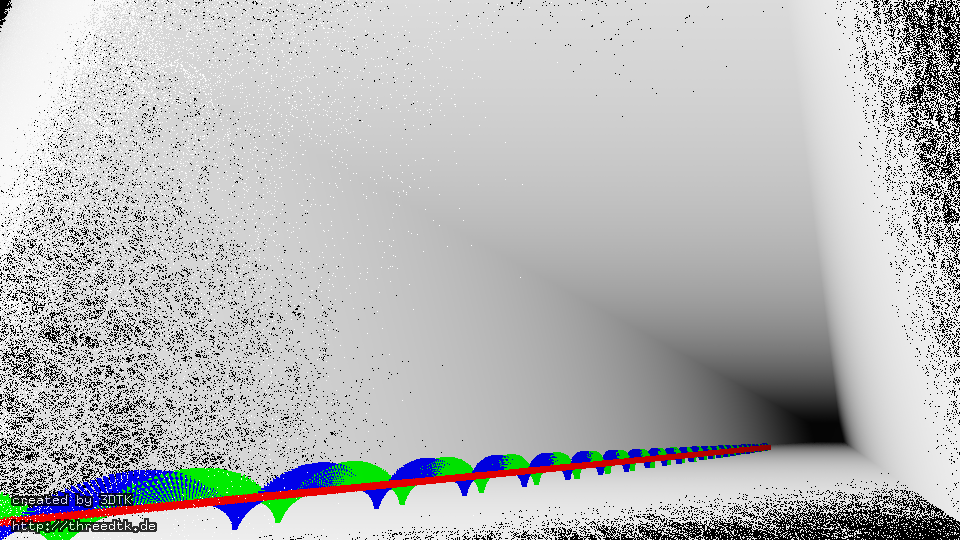
\includegraphics[width=0.495\textwidth]{images/perfect_bottom}\hfill
	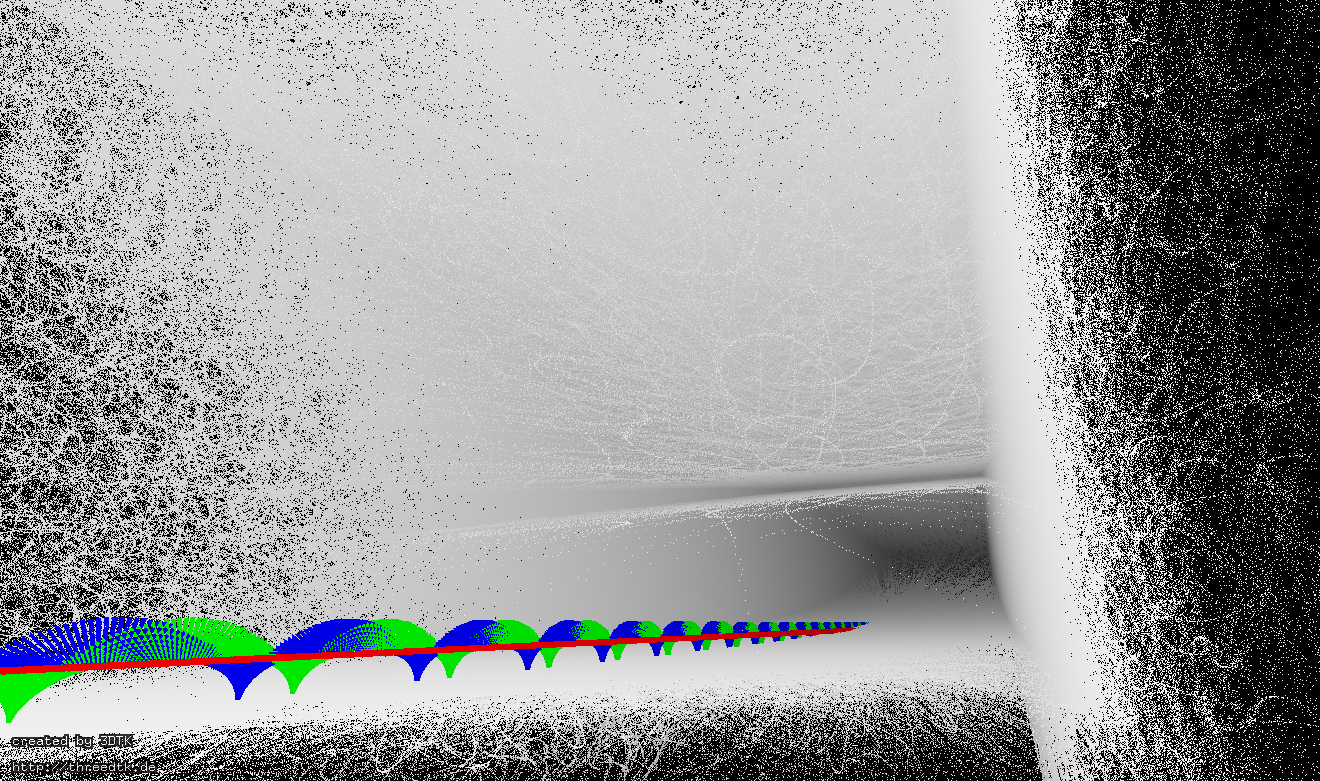
\includegraphics[width=0.495\textwidth]{images/noisy_pose_and_range_bottom}\\
	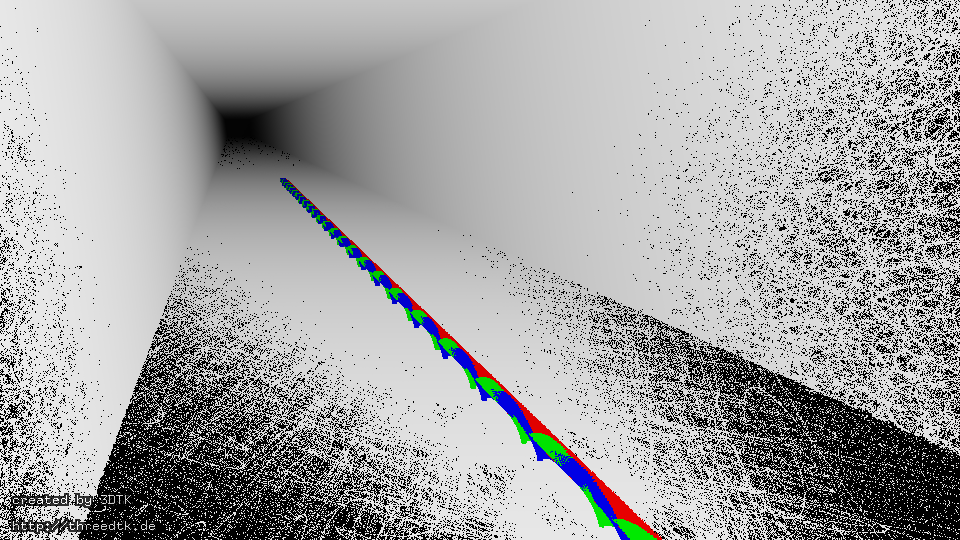
\includegraphics[width=0.495\textwidth]{images/perfect_top}\hfill
	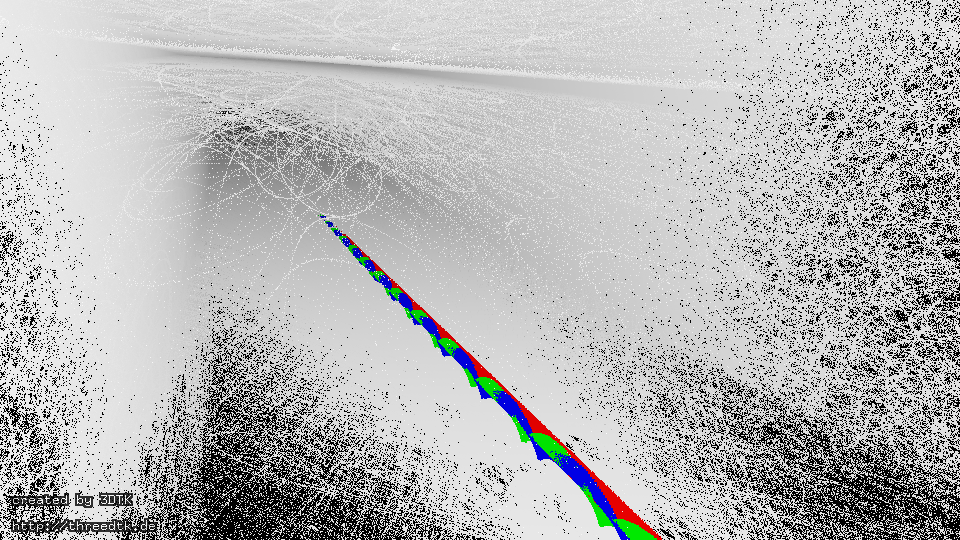
\includegraphics[width=0.495\textwidth]{images/noisy_pose_and_range_top}\\
	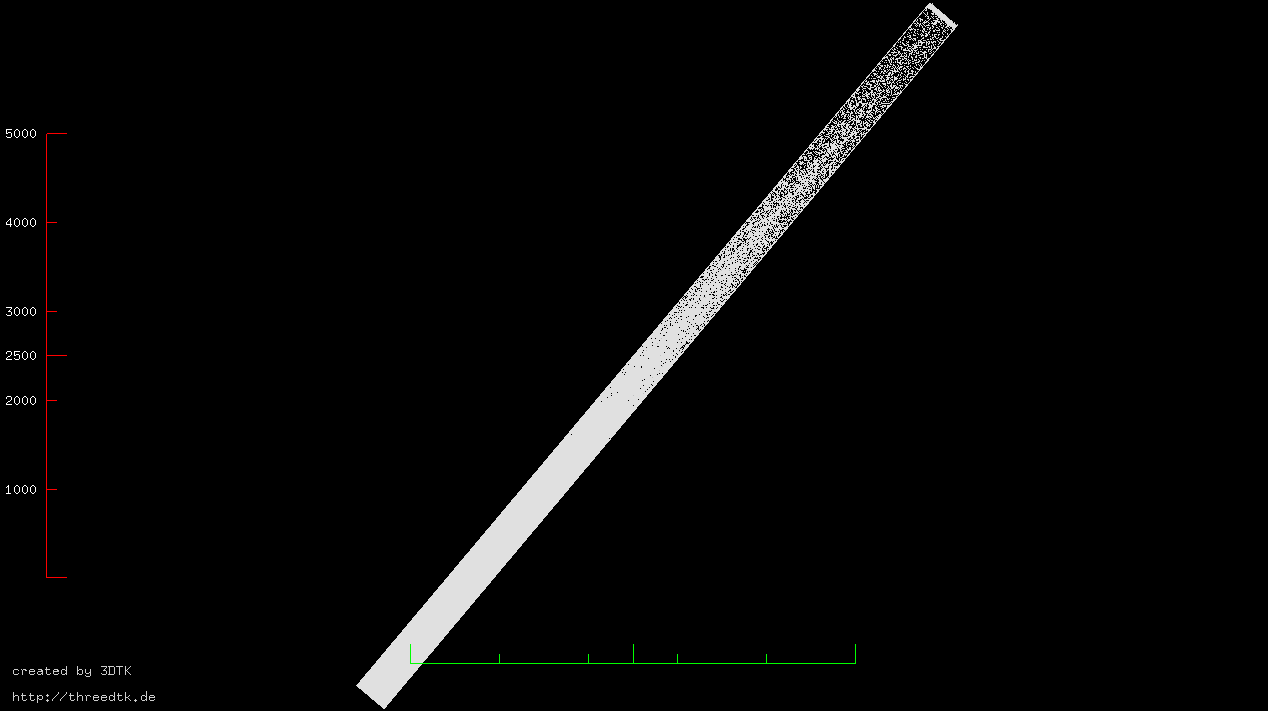
\includegraphics[width=0.495\textwidth]{images/perfect_top_view}\hfill
	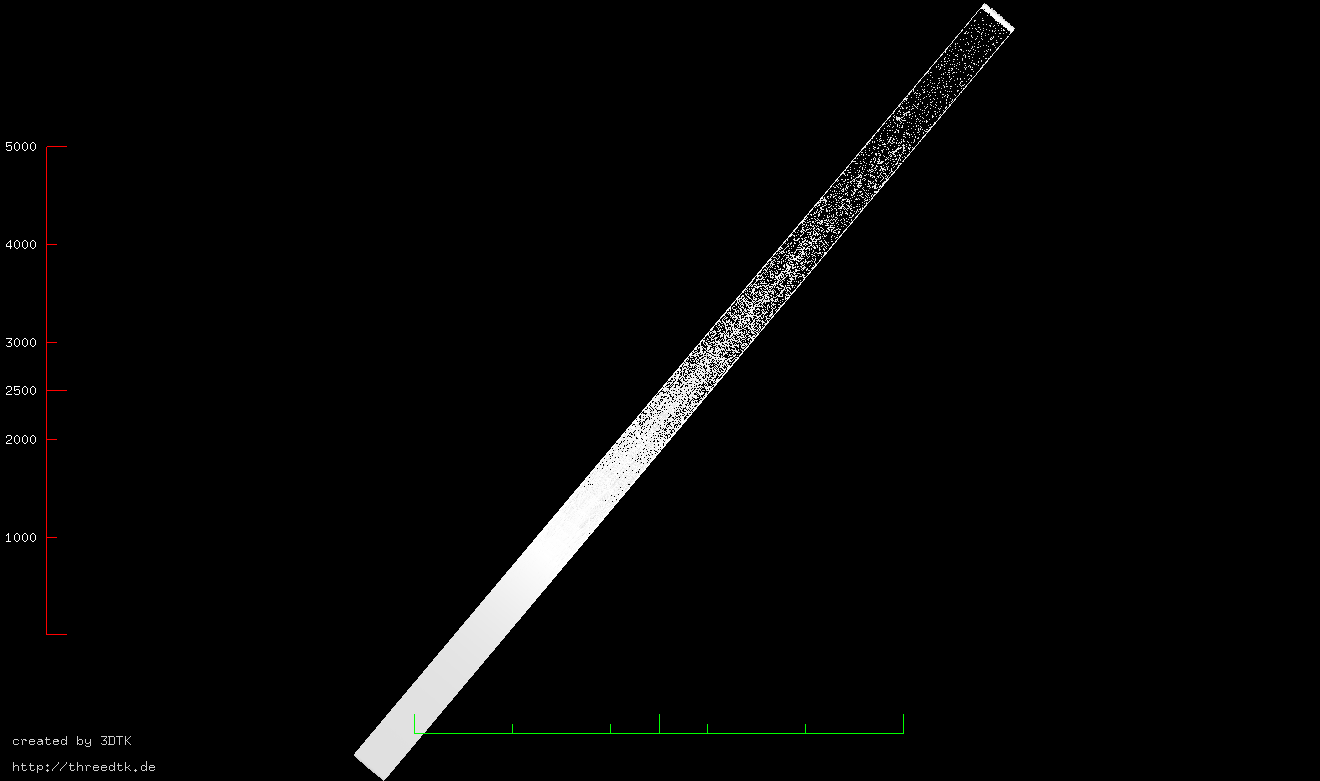
\includegraphics[width=0.495\textwidth, height=0.1825\textwidth]{images/noisy_pose_and_range_top_view}
	\caption{Two simulated datasets of a long hallway of size $\SI{4}{\meter}\times\SI{3}{\meter}\times\SI{100}{\meter}$. Ideal noise free (left), noisy pose ($\mathcal{N}_\varphi = \mathcal{N}_\psi(\mu = 0.0001, \sigma= 0.00001)$) and noisy range measurements ($\mathcal{N}_r(\mu = 0, \sigma = 0.001)$) (right). 
	The normal distributions are define in such a way, that in the resulting dataset plane detection is still possible.}
	\label{fig:simulatedDatasets}
\end{figure*}

\begin{figure*}
	\centering
	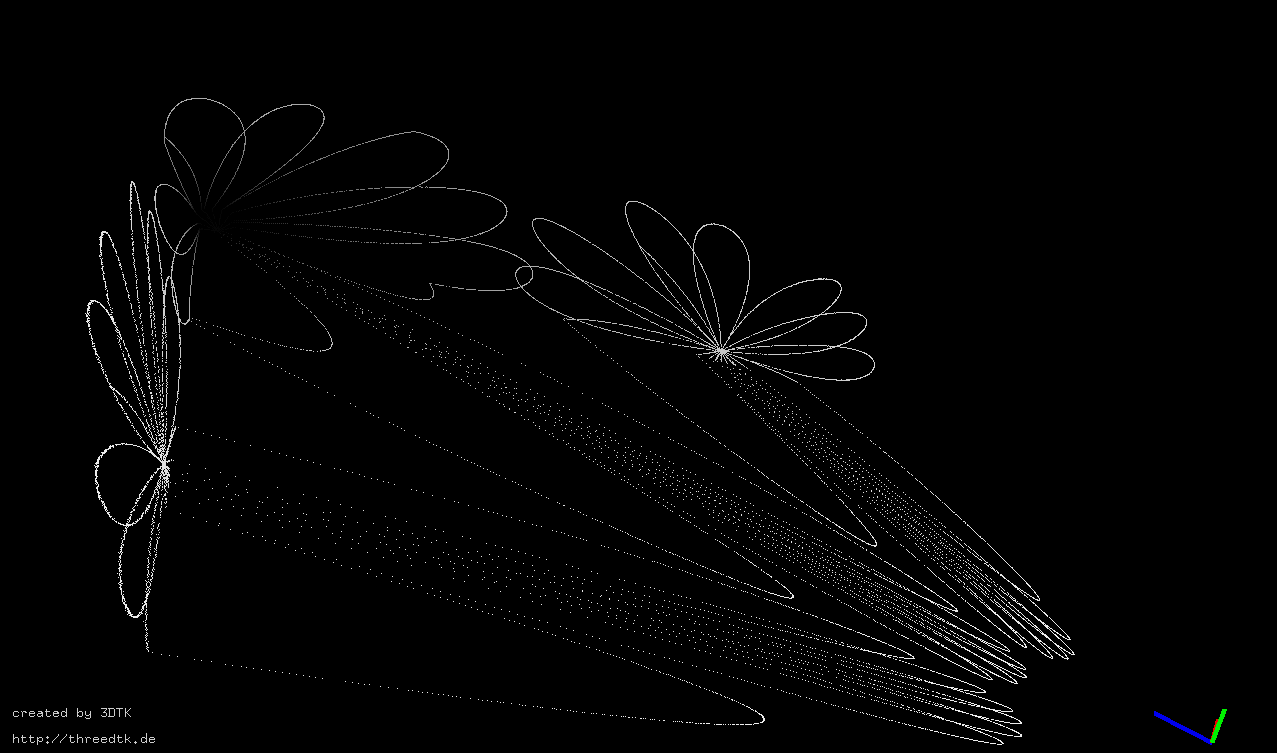
\includegraphics[width=0.495\textwidth]{images/sim_frame_00.png}\hfill
	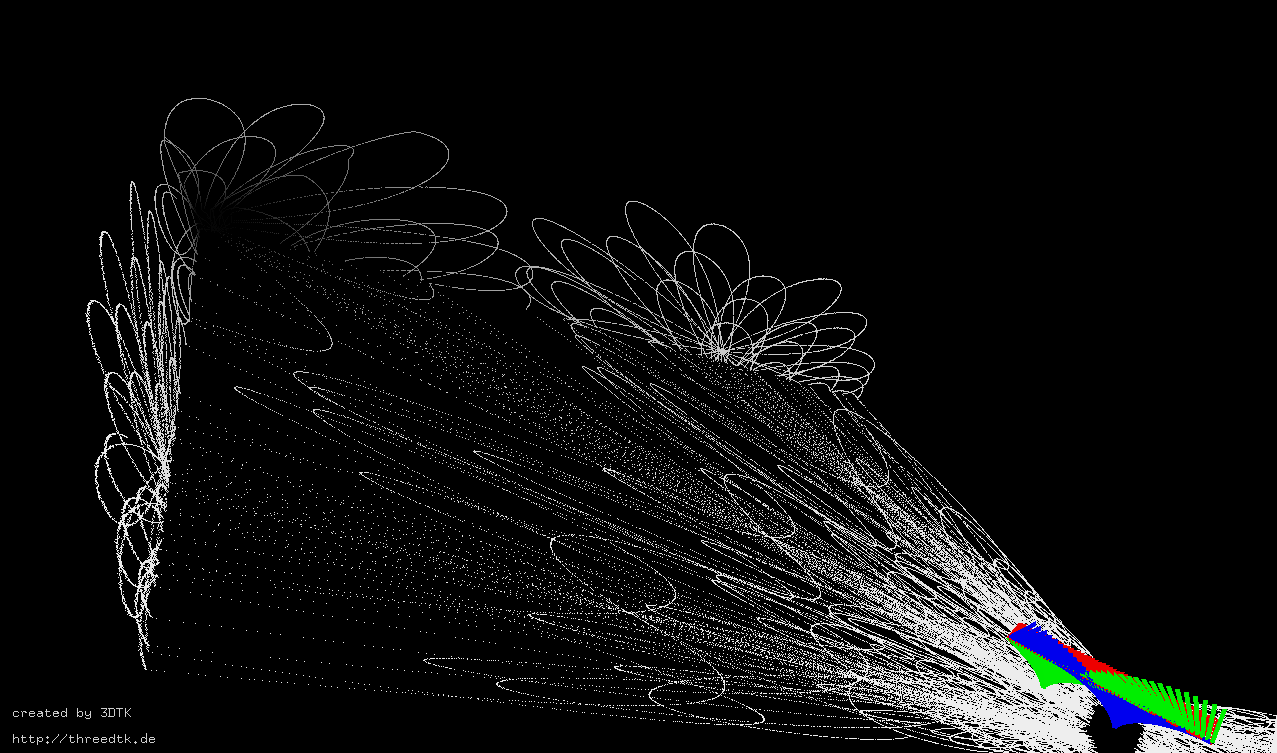
\includegraphics[width=0.495\textwidth]{images/sim_frame_02.png}\\
	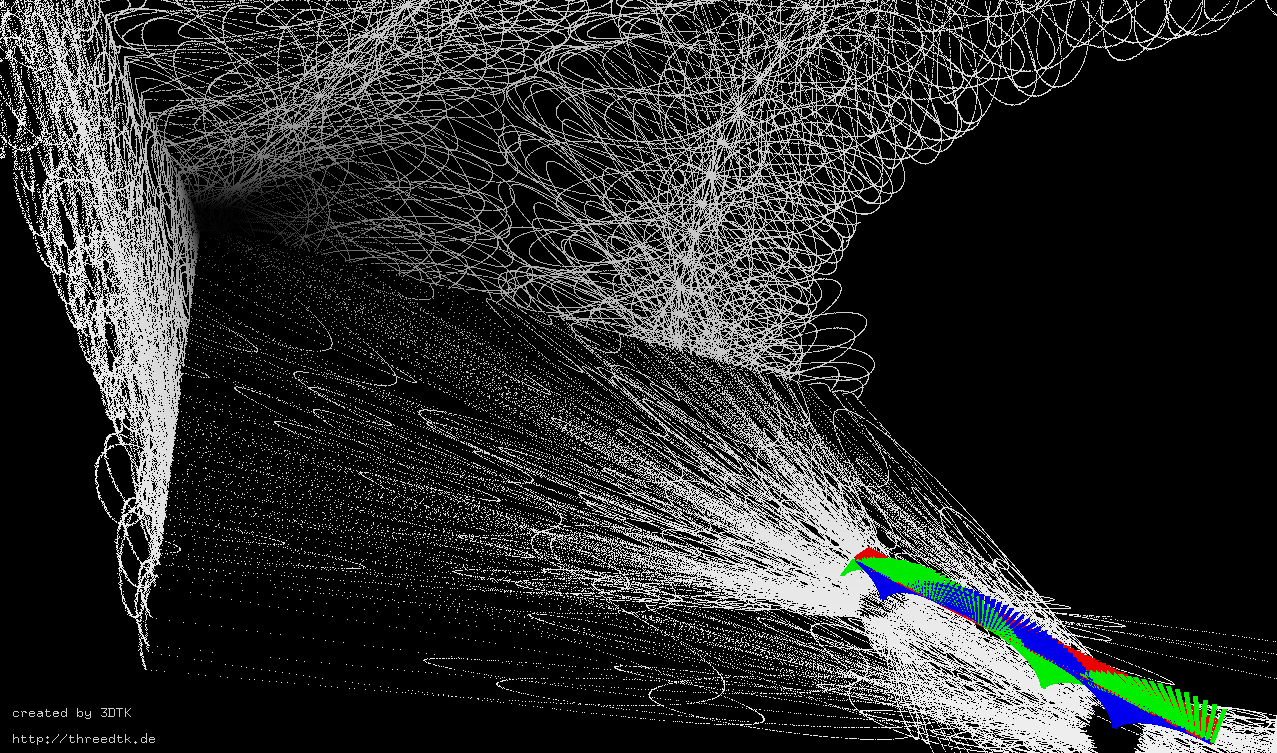
\includegraphics[width=0.495\textwidth]{images/sim_frame_06.png}\hfill
	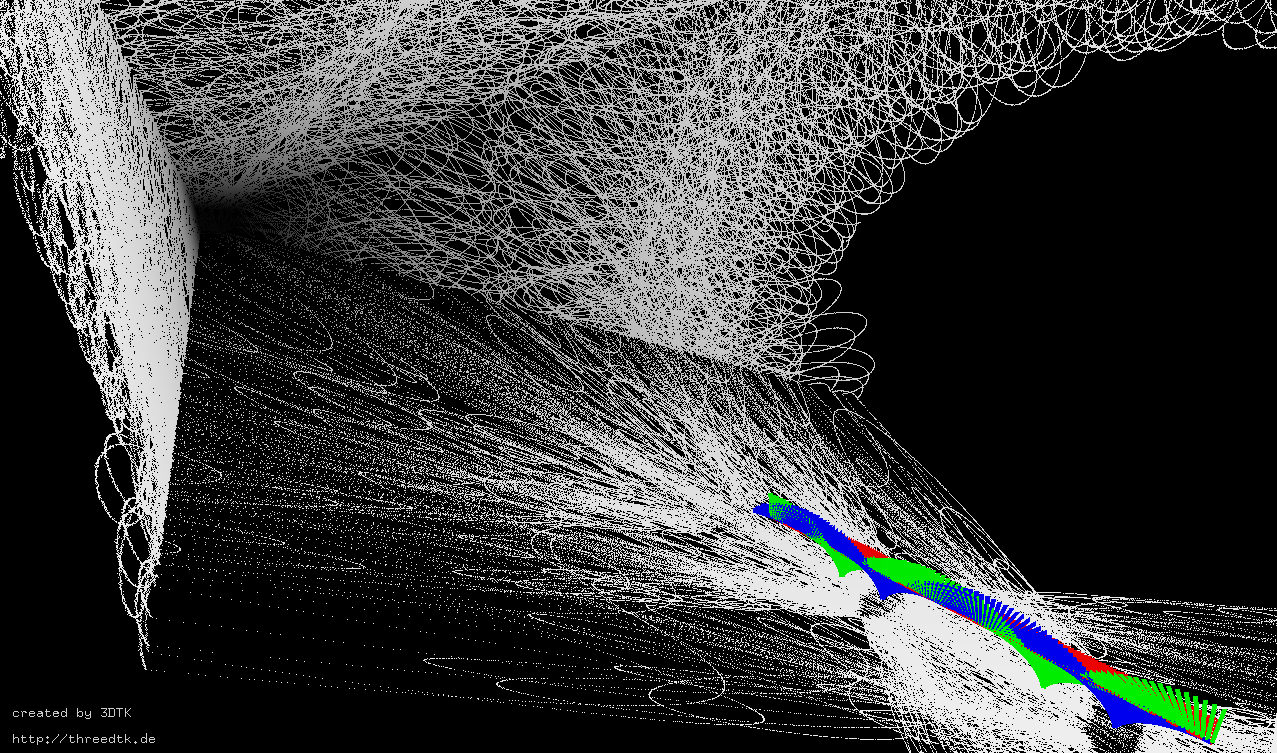
\includegraphics[width=0.495\textwidth]{images/sim_frame_08.png}\\
	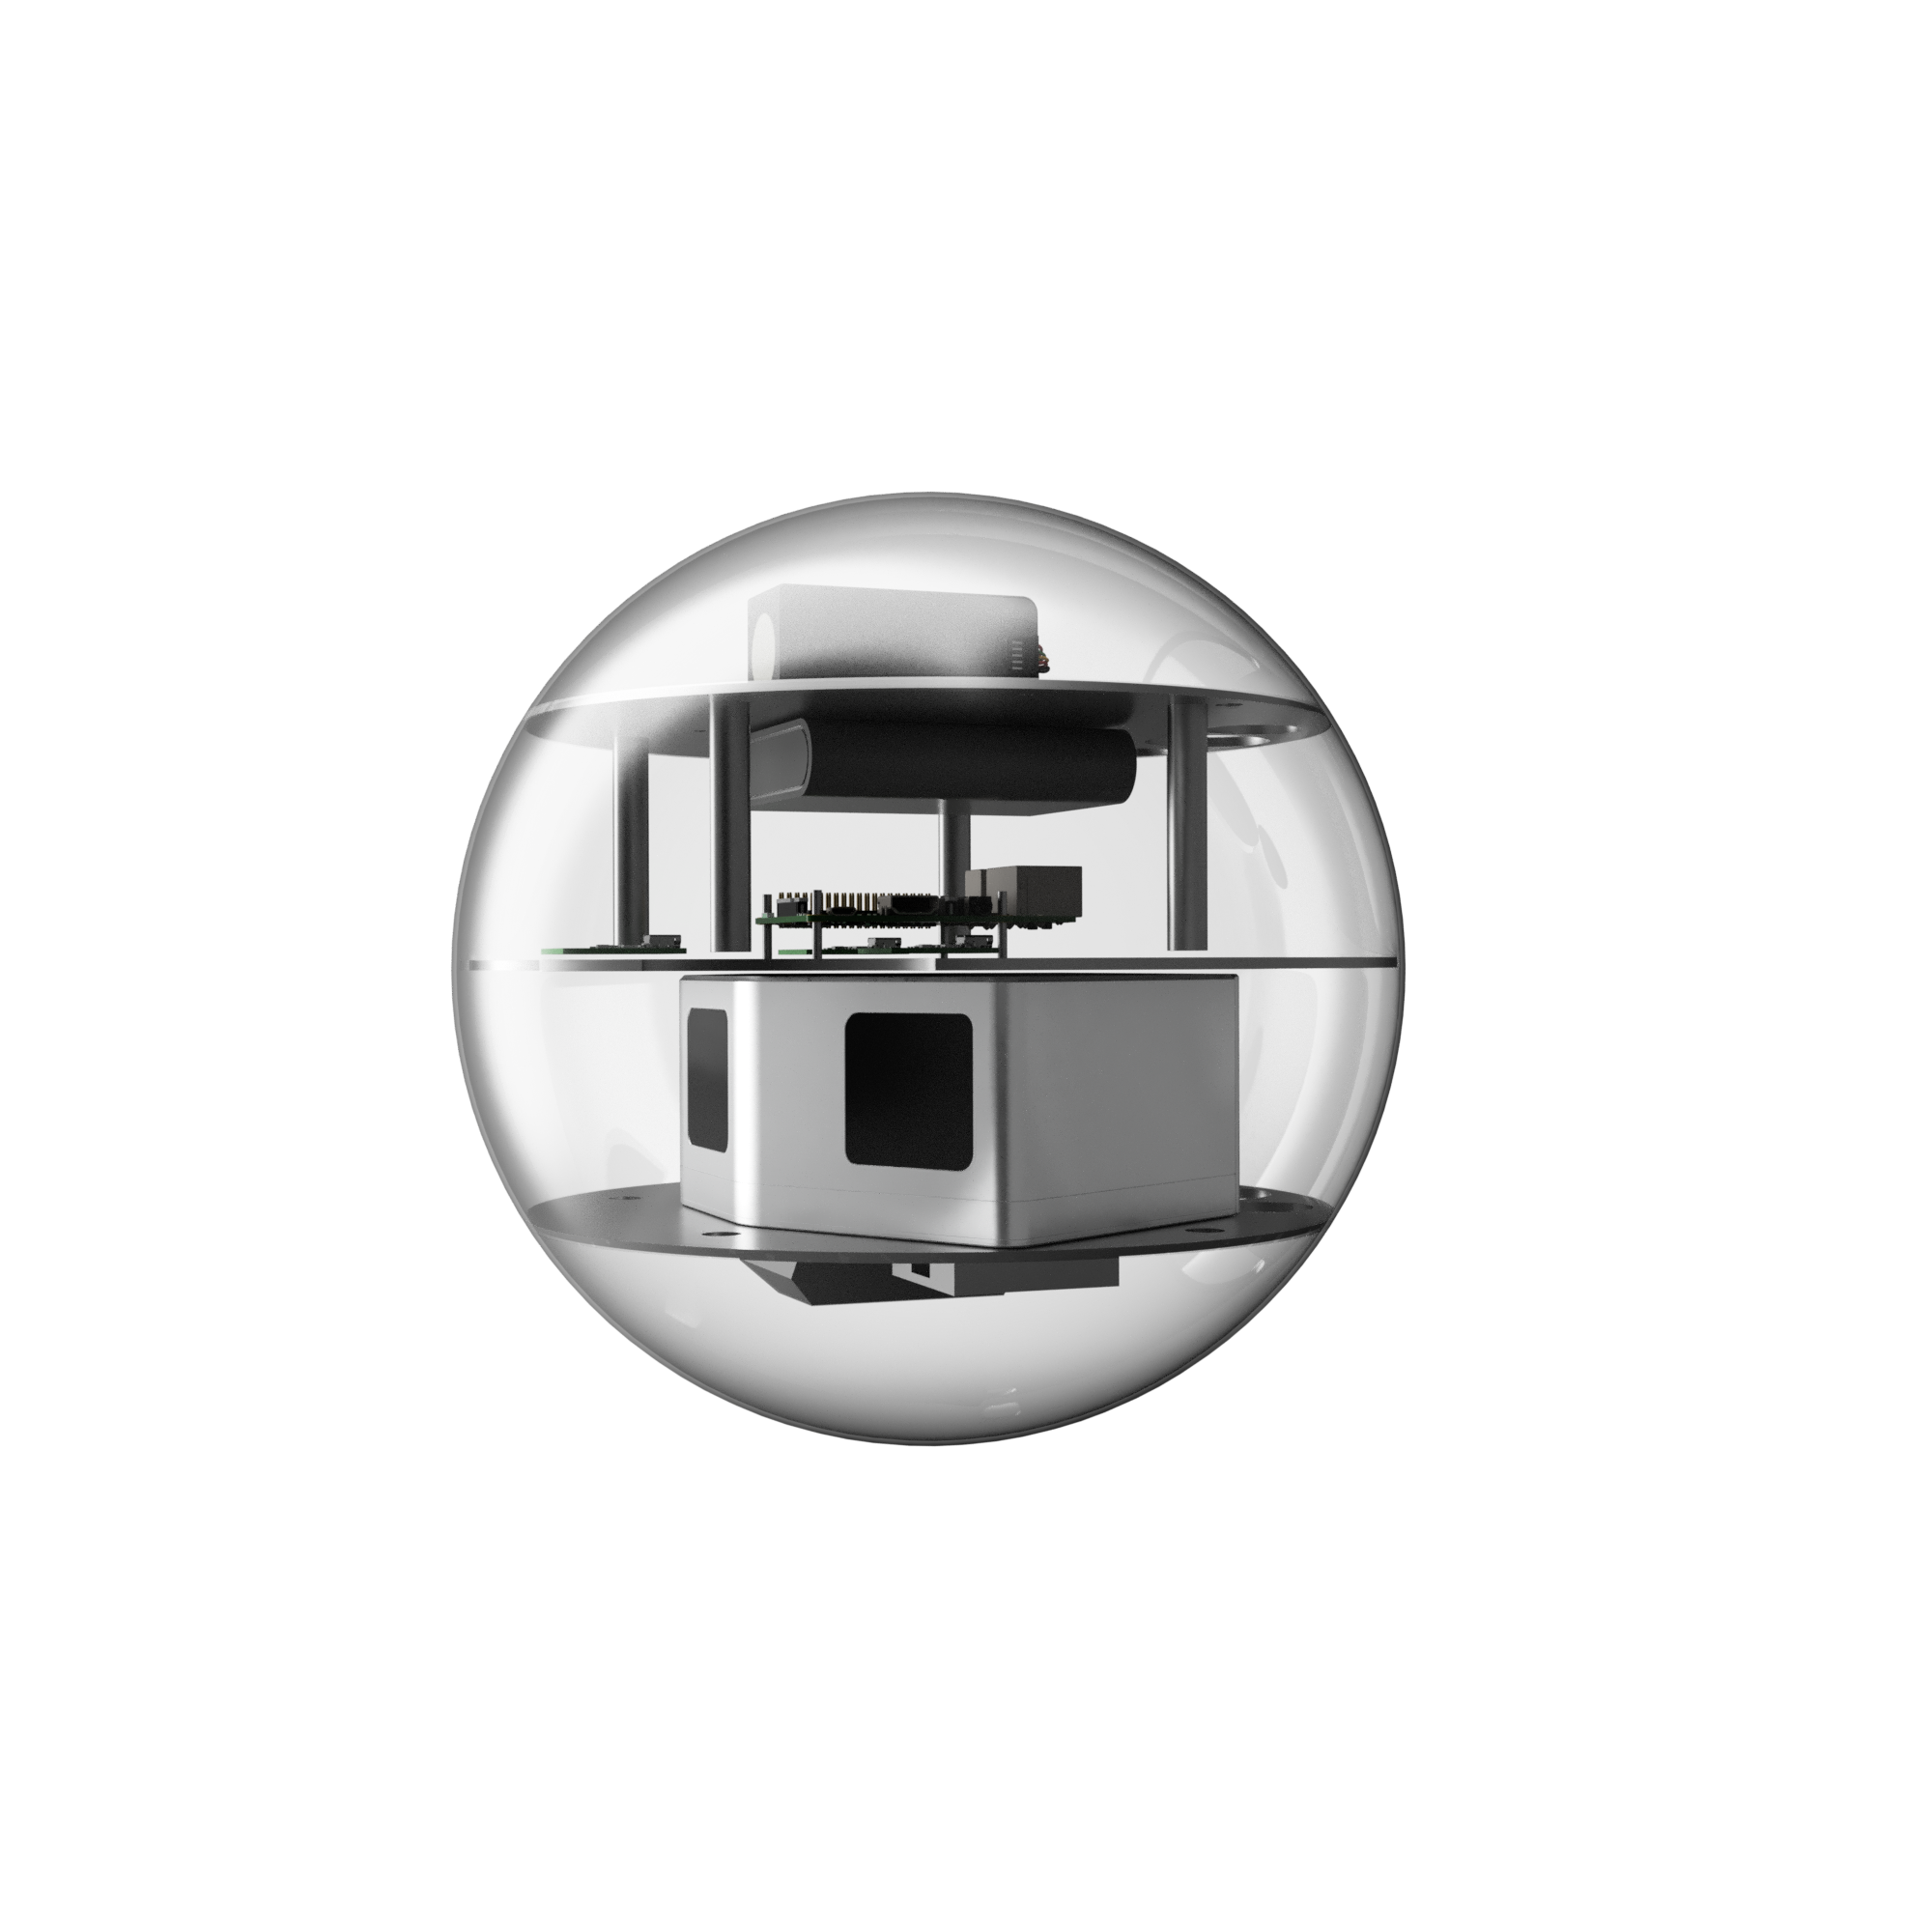
\includegraphics[width=0.495\textwidth]{images/ProtoRoll1.png}\hfill
	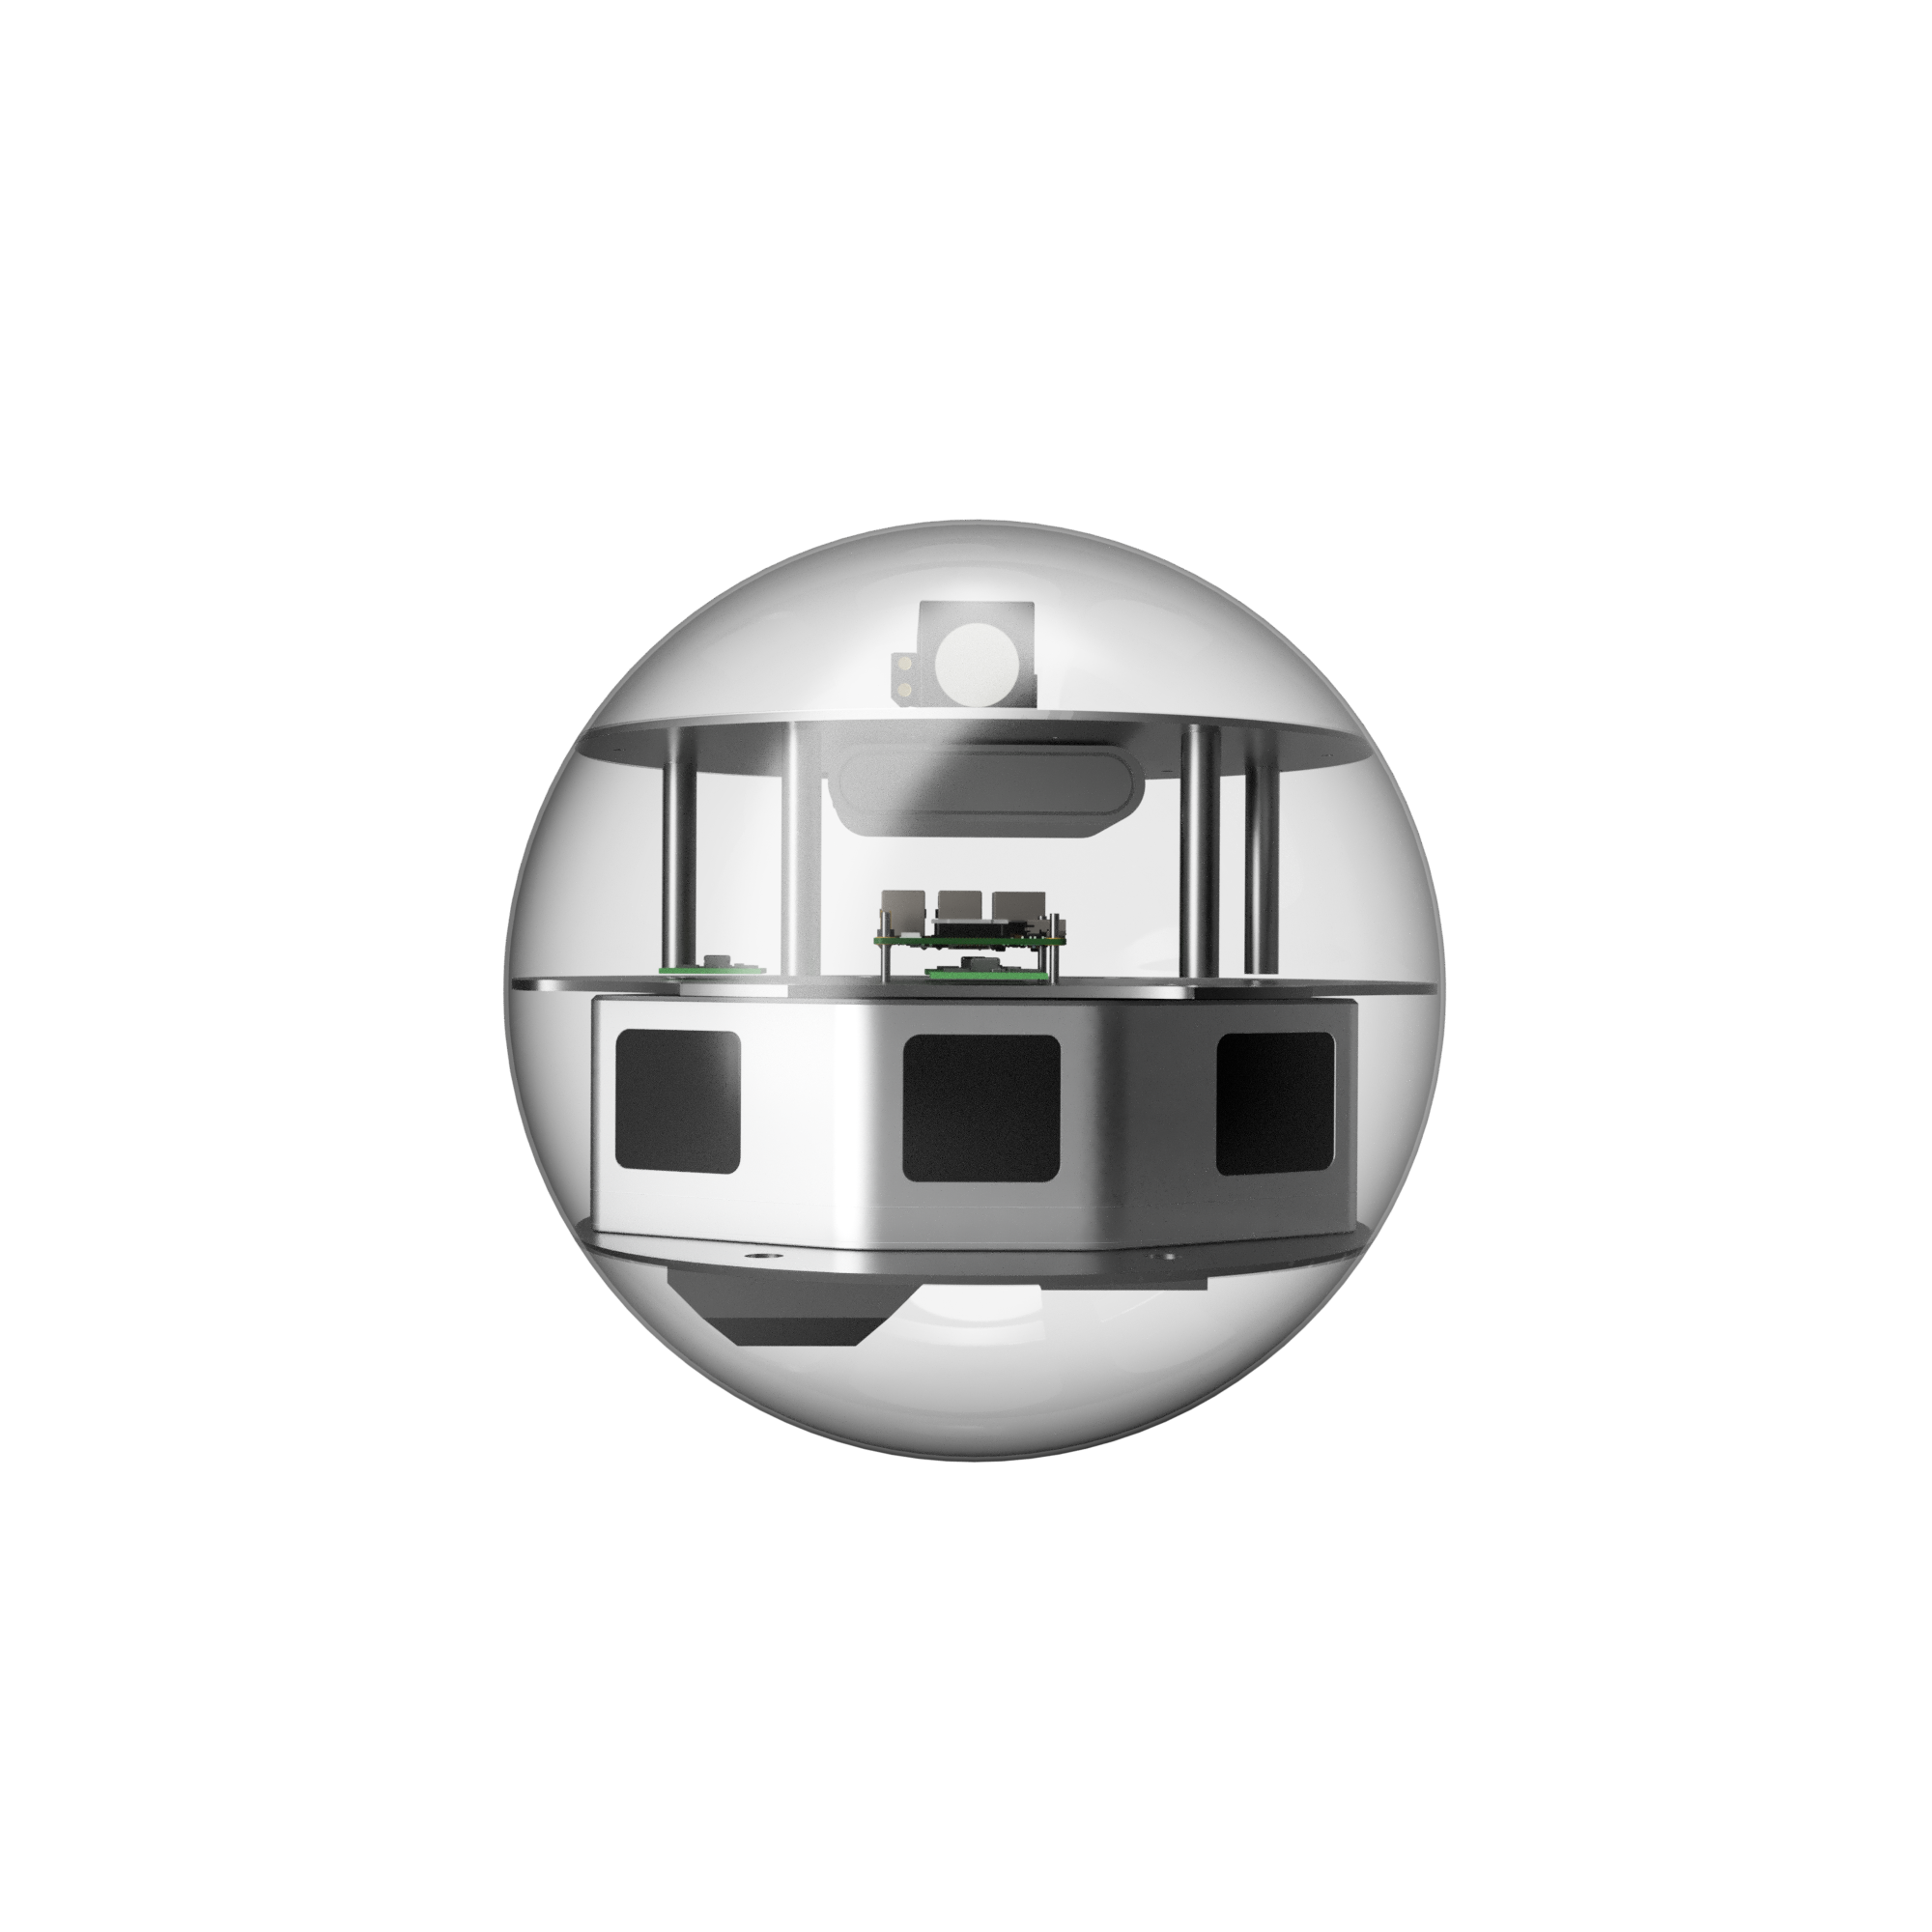
\includegraphics[width=0.495\textwidth]{images/ProtoRoll2.png}
	\caption{Top: Initial sequence of the simulation of the ideal dataset showing the simulated motion of the robot.
	Below: Rendering of the simulated robot, a Livox laser scanner insider a spherical shell.}
	\label{fig:robotRender}
\end{figure*}
